\documentclass[10pt]{report}

%opening
\title{Automated Checking of Implicit Assumptions on Textual Data} 
\author{Radwa Sherif Abdelbar \\
	 Supervisors: Dr. Caterina Urban, Alexandra Bugariu \\ Prof. Dr. Peter M{\"u}ller}
\usepackage{titlesec}
\usepackage{tikz}
\usepackage{natbib}
\usepackage{amsfonts}
\usepackage{amsmath}
\usepackage{stmaryrd}
\usepackage{amsmath}
\usepackage{amsfonts}
\usepackage{listings}
\usepackage{syntax}
\usepackage{algorithm}
\usepackage[noend]{algpseudocode}
\usepackage[T1]{fontenc}
\usepackage{setspace}
\usepackage{graphicx}
\usepackage{url}
\usepackage{pdfpages}
\usepackage{pgfplots}
\lstdefinestyle{mystyle}{
	numberstyle=\small,
	breakatwhitespace=false,         
	breaklines=true,                 
	captionpos=b,                    
	keepspaces=true,                 
	numbers=left,                    
	numbersep=5pt,                  
	showspaces=false,                
	showstringspaces=false,
	showtabs=false,                  
	tabsize=2,
	frame=single
}
\lstset{style=mystyle}

\titleformat{\chapter}{\normalfont\huge\bf}{\thechapter}{20pt}{\huge\bf}
\def\changemargin#1#2{\list{}{\rightmargin#2\leftmargin#1}\item[]}
\let\endchangemargin=\endlist

\begin{document}

\maketitle



\begin{abstract}

\end{abstract}

\chapter{Introduction}

Today, we live in a world that produces tremendous amounts of data on a daily basis. The extensive use of social media websites and the digitization of traditional services such as banking, retail and publishing guarantees the existence of large datasets that are available to service providers. In addition to business, technological advancements have created an abundance of data in many fields of scientific research such as the genomic data created by efficient Deoxyribonucleic acid (DNA) sequencing or raw images of celestial bodies that are captured by modern telescopes \cite{blei2017science}. 

This abundance of data, along with the rapid development in new data science techniques and methods to organize, analyze and detect patterns in large datasets, creates new and unique opportunities for experts in different domains. For example, it enables businesses to predict future customer behavior or medical researcher to associate the presence of a specific gene in the human DNA with susceptibility to certain diseases. 

These advantages, however, are not achieved without challenges or difficulties. The datasets processed by data science algorithms are typically very large in size and could be obtained from various sources or maintained on different machines. For these reasons, they are likely to contain errors and inconsistencies. 

In the field of data science, raw data, that is data as it is collected from the source and stored on some storage medium (e.g. database or cloud), is not usually usable as is. A recent survey among data scientists \cite{kaggle} shows them to cite ``dirty data'' as one of the most challenging aspects of their work. Dirty data, as defined in \cite{dirty-data}, is data that is wrong, missing or not represented according to a known standard such as non-standard representation of time and date.

Before feeding the data into a data science program, it must be cleansed and the erroneous values must be eliminated. Many tools have been introduced to achieve this goal.. [mention some data cleaning tools.] 

In this thesis, we present an approach to detect incorrect input data with respect to a given data science program. Unlike the data-cleaning tools mentioned above, our method does not perform computations on the dataset directly. Instead, we design a static analysis that analyzes the source code of the program in order to find out the implicit assumptions that the program makes about the input data that it reads such that if these assumptions are violated the program will crash. These assumptions represent the pre-conditions that must be satisfied so that the program runs without producing errors. Our analysis will compute an over-approximation of these pre-conditions. In other words, if there is a set of accepted values that will allow the program to run without raising an error, the set of values that our analysis computes will contain all the accepted values, but it might contain some extra values that will cause the program to raise errors. That is, the pre-conditions we compute are necessary but not sufficient for the program to terminate without crashing. 

We then design an input checker that looks for values that violate the assumptions computed by the analysis. If that is the case, the wrong input values are flagged as errors so that the user can correct them. Our approach is advantageous in cases where the data cannot be shared with third parties to perform data cleaning. We implement our analysis and input checker for Python programs and integrate them into a tool that can be used directly by domain experts on their data. 
\begin{lstlisting} [language = Python, label=first, caption=Example of Assumptions on String Data] 
	sequence_length: int = int(input())
	count_a: int = 0
	count_c: int = 0
	count_g: int = 0
	count_t: int = 0
	for i in range(sequence_length):
		base: str = input()
		if base == 'A':
			count_a: int = count_a + 1
		elif base == 'C':
			count_c: int = count_c + 1
		elif base == 'G':
			count_g: int = count_g + 1
		elif base == 'T':
			count_t: int = count_t + 1
		else:
			raise ValueError
			
\end{lstlisting} 

To elaborate further on what we aim to achieve in this thesis, let us examine the program in Listing 1. This program aims to read a DNA sequence and count the frequency of occurrence of each nucleotide. It first reads the length of the sequence (line 1), then since the only possible nucleotides in a DNA sequence are represented by the letters A, C, G and T, it sets a frequency counter for each of these nucleotides (lines 2-5). Then the program iterates through the sequence, reading one letter per line and incrementing the corresponding counter variable. If it encounters a letter that is neither A, C, G or T, it raises an exception because it \textit{assumes} that, in an ideal scenario, no value in the input file will be outside this set of letters.  

Our aim, thus, is not to perform computations on the input data based on the known fact that the human DNA contains only A, C, G and T bases and to cleanse the wrong values. Rather, we turn our attention to the program that will run on the data and try to answer the question: what does this program \textit{assume} about its input data such that if those assumptions are not fulfilled, the program will raise an error? For our analysis to compute a successful over-approximation, it must always include the character `A', `C', `G' and `T' in the set of accepted values it produces. However, it may include some other values as well. 

In section \ref{theoretical}, we present the theoretical aspects upon which the work of this thesis is based. In section \ref{analysis}, we explain the design of our static analysis and its different components in more detail. In section \ref{implementation}, we give an overview of how our analysis and input checker were implemented and integrated into an IDE plug-in. We evaluate the work achieved in this thesis in section \ref{evaluation} and, finally, the conclusion and possible future work are to be found in section \ref{conclusion}. 

\section{Theoretical Background} \label{theoretical}
\subsection{Static Analysis}
[Explain what static analysis is on a high level, what it's used for, the ways to do it]
\subsection{Abstract Interpretation}
[Explain briefly abstract interpretation and the advantages of using it in static analysis, element of an abstract domain.]

\section{Previous Work and Contribution}

We build our approach on the work done in \cite{madelin}. This work was focused on inferring assumptions on numerical values in terms of types, ranges and simple relations. They designed a type domain which we also use in this thesis and describe in section \ref{types} and a simple relations domain to keep track of relations between numerical variables such as $ x \leq y $. For ranges the used the well-known Interval Domain \cite{cousot}. They also used a stack mechanism to store assumptions collected about the input values by the domains they employed. 

Since we would like to analyze more evolved code examples that contain assumptions on both numerical and string values, such as Listing \ref{first}, we take a more generic approach to the problem in this thesis. We design our static analysis to be a generic framework which can employ any existing value domain to keep track of assumptions on the input data. This way, we can employ more powerful domains, for example the Octagon Domain which we use in this thesis, to keep track of relations between numerical variables and we can also keep track of assumptions on different types of variables, for instance numerical and string variables, at the same time. We also extend the stack mechanism used in \cite{madelin} to be more generic and to keep track of assumptions from different domains simultaneously.  

\chapter{Static Analysis Design} \label{analysis}

\section{Concrete Domain} \label{concrete}

To define our concrete domain, we first define the following sets:
\begin{itemize}
	\item $\mathcal{L}$: the set of all program points in the program being analyzed. 
	\item $\mathcal{S}$: the set of all possible string values. 
	\item $\mathcal{V}$: the set of all program variables.
	\item$\wp(\mathcal{V} \rightarrow \mathcal{S})$: the set of environments mapping program variables to their possible values. 
	\item $\wp(\mathcal{S})^{*}$: the list of values read as input from one program point onwards.  
\end{itemize}

We can then define our concrete domain as follows: 
\begin{center}
$\mathcal{L} \rightarrow \wp(\mathcal{V} \rightarrow \mathcal{S}) \times \wp(\mathcal{S})^{*}$
\end{center}

As indicated by the formula, our  concrete domain maps a program point to a set of mappings of program variables to the values they are allowed to take and a list of input values which the program reads from this point onwards. Specifically, given a program, its concrete semantics is the set of values that its variables are allowed to take and the list of input values that it is allowed to read so that it terminates without errors.   

\section{The Assumption Abstract Domain} \label{assumption-domain}
We use the theory of Abstract Interpretation \cite{cousot} to design an abstract domain that over-approximates the concrete semantics defined in the previous section. In this context, over-approximation means that the constraints inferred by the analysis are necessary but not sufficient for the program to run without producing an error. If the input values violate those constraints, the program is guaranteed to produce an error. We guarantee an absence of false-positives. However, if the input values satisfy all the constraints, the program might still produce an error. Our static analysis works backwards by starting at the final state of the program and analyzing all the execution paths of the program till it reaches the initial state.  

To examine the properties of our domain, let us consider the program in Listing 2, which performs the same operation as Listing 1, namely reading a DNA sequence and counting the frequency of every nucleotide, but on multiple sequences separated by a '.' or '\#' character. On line 1, the number of sequences is read. Lines 3 and 4 assert that we have at least one sequence in the file. Another addition in Listing 2 is the check that the sequence length is not greater than some maximum length on lines 7 and 8. 

There are multiple ways in which this program can produce an error. On line 1 if the value read cannot be cast to an integer, a error will be raised by Python. If the number of sequences is not positive (line 3), the length of each sequence is greater than the designated maximum sequence length, the sequence contains characters other than A, C, G and T (lines 15 through 24) or if the separator character is not a hash or a dot (line 26), the program raises a ValueError explicitly. 

It is obvious from this example that we need to track information about both numerical values and string values if we are to compute the set of allowed input values to this program. For examples we need to ensure that the relation $sequence\_length > max\_length$ holds and that the variable $base$ has only the characters in the set $\lbrace'A', 'C', 'G', 'T' \rbrace$. This cannot be achieved by running a conventional static analysis using only one abstract domain.

\begin{lstlisting} [language=Python, label=, caption=Example of Assumptions on both String and Numerical Data]
	number_of_sequences: int = int(input())
	max_length: int = int(input())
	if number_of_sequences <= 0 :
		raise ValueError("Expecting at least one DNA sequence")
	for s in range(number_of_sequences):
		sequence_length: int = int(input())
		if sequence_length > max_length:
			raise ValueError
		A_count: int = 0
		C_count: int = 0
		G_count: int = 0
		T_count: int = 0
		for i in range(sequence_length):
			base: str = input()
			if base == 'A':
				A_count: int = A_count + 1
			elif base == 'C':
				C_count: int = C_count + 1
			elif base == 'G':
				G_count: int = G_count + 1
			elif base == 'T':
				T_count: int = T_count + 1
			else:
				raise ValueError
		separator: str = input()
		if separator == '.' or separator == '#':
			pass
		else:
			raise ValueError
\end{lstlisting}



Our abstract domain, which we call the Assumption Domain, is a generic domain that allows for the approximation of multiple program properties simultaneously. It is parametrized by a list of abstract domains which are independent of one another. For each step of the analysis, the Assumption Domain invokes the corresponding operator or transformation on each domain independently. We define a $ SUBD $ to be a family of domains that can be used in our analysis. Any value domain can be a member of this family given that it define extra operators that are described in \ref{sub-domains}. The Assumption Domain uses these domains to keep track of assumptions on the values of program variables. For example, in the case of , we can use the Octagons Domain \cite{octagon} to keep track of the relations between numerical variables such as $sequence\_length \leq max\_length$ and the Character Inclusion Domain \cite{character} to keep track of the characters of the variable $base$.

Going back to Listing 2, if we trace a backward static analysis from line 24 to line 15 using the Character Inclusion Domain as a sub-domain, we will get that the variable $ base $ is allowed to contain only the characters 'A', 'C', 'G' and 'T'. When this variable is read as input on line 14, we need to store the assumption in some data structure. The same applies for the variable $ sequence\_length $. Tracing the analysis backwards using the Octagon Domain will give us the constraint $ sequence\_length \leq max\_length $. On line 6, when the variable is read as input, this constraint must be stored in a way that preserves its order among other inputs that the program reads in the course of its execution. More specifically, we need a data structure in which the assumptions about $ sequence\_length$ appear before those about $ base $.  We also need a data structure that indicates how many times an input value is read. For example, it needs to show that the variable $ base $ is read $ sequence\_length $ number of times. 

In our case, we choose this data structure to be a stack, in which every layer represents a scope of the program. Whenever the analysis enters a new branch or a loop, a new layer is pushed onto the stack. Inside of this scope, whenever a variable is read as input, we store its constraints in the top layer of the stack. When exiting a branch or a loop, the top layer is popped from the stack and combined with the layer below it in such a way that the assumptions appear in the order in which the inputs are read. In the case of exiting a loop, we define a mechanism to indicate how many times a group of assumptions are repeater. This way, at the end of the analysis, the stack will contain all the assumptions on the input value of the program in the correct order. We define the stack with further detail in section \ref{stack}. 

Given the previously mentioned properties, we introduce our domain formally below. \\
  

We define $STACK$ to be a set of all possible stacks which store assumptions on input values of the program.

We use the notation $ (X_{i})_{i=1}^{n} $ throughout this thesis to indicate a list of length $ n $.  \\

We can define the Assumption Domain formally as follows: \\
\begin{center}
	$D \equiv SUBD^{n} \times STACK$\\	
\end{center}
\begin{itemize}
	\item An element $d \in \textsl{D} = \lbrace ((S_{i})_{i=1}^{n}, Q) \vert S_{i} \in SUBD \wedge Q \in STACK \rbrace$. Every element of this domain consists of a sequence of instances of sub-domains and a stack.
	\item A concretization function $\gamma_{D}(d) =( \bigcap\limits_{i=1}^{n}\gamma_{S_{i}}(S_{i}), \gamma_{STACK}(Q)).$ 
	 
	\item A partial order $\sqsubseteq_{D}$ such that $ ((S_{1,i})_{i=1}^{n}, Q_{1}) \sqsubseteq_{D} ((S_{2, i})_{i=1}^{n}, Q_{2}) \Longleftrightarrow \bigwedge\limits_{i=1}^{n}(S_{1i} \sqsubseteq_{S_{i}} S_{2i}) \wedge Q_{1} \sqsubseteq_{STACK} Q_{2} .$ An element $ d_{1} $ of $ D $ is small than or equal to another element $ d_{1} $ if and only if $ d_{1} $ represents a set of allowed input values that is smaller than or equal the set allowed input values by $ d_{2} $. 
	\item A minimum element $\bot_{D} = ((\bot_{S_{i}})_{i=1}^{n}, \bot_{STACK})$. This elements represents a state where there are no possible input values that are acceptable by the program. 
	\item A maximum element $\top_{D} =  ((\top_{S_{i}})_{i=1}^{n}, \top_{STACK})$. This represents the set of all possible input value without any constraints. 
	\item A join operator $\sqcup_{D}$ such that $ ((S_{1,i})_{i=1}^{n}, Q_{1}) \sqcup_{D} ((S_{2,i})_{i=1}^{n}, Q_{2}) = (((S_{1,i} \sqcup_{S_{i}} S_{2,i})_{i=1}^{n}, Q_{1} \sqcup_{STACK} Q_{2}))$. When joining two paths of the analysis, we must join the assumptions computed by the analysis on the program variables. 
	\item A meet operator $\sqcap_{D}$ such that $ ((S_{1,i})_{i=1}^{n}, Q_{1}) \sqcap_{D} ((S_{2,i})_{i=1}^{n}, Q_{2}) = (((S_{1,i} \sqcap_{S_{i}} S_{2,i})_{i=1}^{n}, Q_{1} \sqcap_{STACK} Q_{2}))$. Similar to the join, the meet operator is applied pair-wise to all sub-domains and the stack.
	\item A backward assignment operator $\llbracket X:=aexpr \rrbracket ((S_{i})_{i=1}^{n}, Q) =  ((\llbracket X:=aexpr \rrbracket(S_{i}))_{i=1}^{n}, \llbracket X:= expr \rrbracket(Q)).$ The backward assignment operator is applied element-wise to every sub-domain and to the stack. 
	\item A filter operator $ \llbracket bexpr \rrbracket ((S_{i})_{i=1}^{n}, Q) =  ((\llbracket bexpr \rrbracket(S_{i}))_{i=1}^{n}, \llbracket bexpr \rrbracket(Q)). $ The filter operator is applied element-wise to every sub-domain and to the stack.
	\item A widening operator $\nabla_{D}$ such that $ ((S_{1,i})_{i=1}^{n}, Q_{1}) \nabla_{D} ((S_{2,i})_{i=1}^{n}, Q_{2}) = $ $ ((S_{1, i} \nabla_{S_{i}} S_{2,i}), Q_{1} \nabla_{STACK} Q_{2}) .$ Similar to the join and meet, widening is applied pair-wise between the sub-domains and the stack. 
\end{itemize}

\subsection{Sub-domains} \label{sub-domains}

As mentioned in the previous section, our Assumption Domain can make use of any existing abstract domain in order to track assumptions on input data. However, in order for this setting to work effectively, we need to define some extra operators for existing abstract domains. 

$SUBD$ is the family of abstract domains which are capable of keeping track of constraints on variables. The variables are either program variables or special variables that represent an input value. An element $F \in SUBD$ is an abstract domain whose concretization function $\gamma_{F}$ operators $\sqcup_{F}, \sqcap_{F}, \sqsubset_{F}, \nabla_{F}$, backward assignment and filter are already defined.
 
The domains used in our analysis are required to define a special \textit{replacement} operator $ \mathcal{R}_{F}(v, f, x) $ that, when an input value is read and stored in variable $ v \in \mathcal{V} $, introduces some special variable $ x $ into element $ f $ of a relational domain $ F $ that denotes this input value and its relation to other variables. This newly introduced variable has to provide information on the order in which an input value was read with respect to other input values in the program. One possible definition for a replacement operator is to replace a variable that is read as input with a special variable $ l_{i} $ that represents the program point $ i $ at which it is read. In this case the operator is $ \mathcal{R}_{F}(v, f, l_{i}) $. 

 
If a program reads inputs from two different paths and these paths are to be joined at some point in the analysis, relational domain elements resulting from these two paths will contain different variables representing the inputs read on these paths. For this reason, we require the sub-domains to define a special operator $ \mathcal{U}(f_{1}, f_{2}) $ that unifies the environment of two elements of a relational domain. From the perspective of our analysis, we do not care about the particular variable that represents an input, but rather about the order in which these input are being read in their respective paths. The unification operator needs to ensure that the constraints on two input value read in the same order on two different paths can be joined successfully. An illustrative example on the replacement and unification operators can be found in section \ref{octagon} where we refer to the Octagon Domain.

\subsection{The Stack} \label{stack}

The stack used in our analysis follows the intuitive definition of a stack. It is composed of layers and defines push and pop operations. To introduce our stack, we need to define a set $B = \lbrace (l, (c_{i})_{i=1}^{n})\ \vert \ l \in \mathcal{L} \wedge \exists_{F_{in} \in SUBD_{in}} c \in F_{in} \rbrace \cup \lbrace \star \rbrace$ which is either a sequence of constraints from any domain in $SUBD$ associated with a specific program point or a constraint represented by $ \star $ which is an empty constraint and is used to indicate a lack of information on what constraints are placed on input values. For example, in Listing 2, an element $(l7, (int, l7 \leq l2)) \in B$ would indicate that the value read from program point 7 is of type integer and is less than the value read form program point 2.

We then define the set of stack layers $I  = \lbrace  m \times (a_{i})_{i=1}^{k}\ \vert m \in \mathbb{M}\ \wedge \ a_{i} \in I \cup B \rbrace$ as a set of possibly repeated constraints on the input data, where $ \mathbb{M} $ is a set of multipliers that indicate how many time the constraints in the list are repeated. A multiplier is either an expression or an integer. For clarity, we express a list of constraints of length $ k $ that is repeated $ m $ times using the notation $ m \times (a_{i})_{i=1}^{k} $. We define a concretization function as well as join, meet and widening operators for the stack layers before we proceed to define them for the whole stack. 

\begin{itemize}
	\item A concretization function $ \gamma_{I} $ is defined recursively as follows:
		\begin{itemize}
			\item $ \gamma_{I}(\star) = \mathcal{S}$. An empty constraint indicates that the input value can be anything. 
			
			\item For $ (l, (c_{i})_{i=1}^{n}) \in B $, $ \gamma_{I}((l, (c_{i})_{i=1}^{n})) = \gamma(c_{1}) \cap ... \cap\gamma(c_{n}) $. A tuple of constraints associated with one program point concertizes to any value that satisfies all of the constraints of this tuple.  
			
			\item For $ m \times (a_{i})_{i=1}^{k} \in I $, $ \gamma_{I}(m \times (a_{i})_{i=1}^{k}) = [\gamma_{I}(a_{1}),.., \gamma_{I}(a_{k})]^{m}$. To concertize a constraint in the set $ I $, the concretization function is applied recursively to its list of constraints, then the result is repeated as many times as the value of its multiplier. 
		\end{itemize}
	\item A partial order $ \sqsubseteq_{I} $:
	\begin{itemize}
		\item For any $ b \in B,\ b \sqsubseteq_{I} \star$. 
		\item For $(l_{1}, (c_{1,i})_{i=1}^{n}), (l_{2}, (c_{,2i})_{i=1}^{n}) \in B$, the partial order is given by $ \bigwedge\limits_{i=1}^{n} c_{1,i} \sqsubseteq_{I} c_{2,i} $. We take the conjunction of the pair-wise order of the elements of the two tuples. 
		\item For $ m \times (a_{1,i})_{i=1}^{k}, m \times (a_{2,i})_{i=1}^{k}  \in I$, that is, two elements in $ I $ with the same multiplier and the same number of constraints, the order is given by $ \bigwedge\limits_{i=1}^{k}a_{1,i} \sqsubseteq_{I} a_{2,i} $. 
		\item For two elements where one belongs to $ I $ and the other to $ B $, we default to false. 
	\end{itemize}
	
	\item A maximum element $ \top_{I} \equiv 1 \times [\star] .$
	\item A minimum element $ \bot_{I}. $
	\item A join operator $\sqcup_{I}$:
	\begin{itemize}
		\item For $ b \in B,\ b \sqcup_{I} \star = \star$
		\item For $(l_{1}, (c_{1,i})_{i=1}^{n}), (l_{2}, (c_{2,i})_{i=1}^{n}) \in B$, the join is given by $ (min(l_{1}, l_{2}), (c_{1,i} \sqcup c_{2,i})_{i=1}^{n}) $. The soundness proof of this join follows from the soundness of the join operator of the individual domains as follows: $ \gamma_{I}((l_{1}, (c_{1i})_{i=1}^{n})) \cup \gamma_{I}((l_{2}, (c_{2i})_{i=1}^{n})) = (\gamma_{I}(c_{1,1}) \cap ... \cap \gamma_{I}(c_{1, n})) \cup (\gamma_{I}(c_{2,1}) \cap ... \cap \gamma_{I}(c_{2, n})) \subseteq \gamma_{I}(c_{1, 1} \sqcup c_{2, 1}) \cap ... \cap \gamma_{I}(c_{1, n} \sqcup c_{2, n}) $. 
		\item For $ m \times (a_{1,i})_{i=1}^{k}, m \times (a_{2,i})_{i=1}^{k}  \in I$, that is, two elements in $ I $ with the same multiplier and the same number of constraints, the join is given by $ m \times (a_{1,i} \sqcup a_{2,i})_{i=1}^{k} $. The soundness can be proved as follows: $ [\gamma_{I}(a_{1,1}), ..., \gamma_{I}(a_{1,k})]^{m} \cup [\gamma_{I}(a_{2,1}), ..., \gamma_{I}(a_{2, k})]^{m} \subseteq [\gamma_{I}(a_{1,1} \sqcup a_{2, 1}), ..., \gamma_{I}(a_{1, k} \sqcup a_{2, k})]^{m}.$
		\item For $ 1 \times (a_{1, i})_{i=1}^{k_{1}}, 1 \times (a_{2, i})_{i=1}^{k_{2}} \in I $, where $ k_{1} \neq k_{2} $, the join is given by $ m \times (a_{1,i} \sqcup a_{2,i})_{i=1}^{min(k1, k2)} \oplus [\star]$. When joining to elements from $ I $ with different constraint lengths, it is inevitable that we lose some information. The addition of the $ \star $ constraint is an indication that there is at least one input value for which we have no constraints and which can take any possible value. The soundness proof is somewhat similar to the previous point. $ [\gamma_{I}(a_{1,1}), ..., \gamma_{I}(a_{1,k})] \cup [\gamma_{I}(a_{2,1}), ..., \gamma_{I}(a_{2, k})] \subseteq [\gamma_{I}(a_{1,1} \sqcup a_{2, 1}), ..., \gamma_{I}(a_{1, k} \sqcup a_{2, k}), \mathcal{S}].$
	\end{itemize}
	\item A meet operator returns the first element since it is not needed by the analysis for the set $ I $. 
	
	\item A backward assignment operator $ \llbracket X := aexpr \rrbracket $ that is applied individually to constraints belonging to the set $ B $. 
	
	\item A widening operator $ \nabla_{I} \equiv \sqcup_{I} .$
	\item A special replacement operator $ \mathcal{R}_{I} $ that is similar to the $ \mathcal{R}_{F} $ operator defined in the previous section:
	\begin{itemize}
		\item For $ (l, (c_{i})_{i=1}^{n}) \in B$, the replacement operator works as follows: $$ \mathcal{R}_{I}((l, (c_{i})_{i=1}^{n}), v, l_{1}) = (l, (\mathcal{R}_{F}(c_{i}, v, l_{1}))_{i=1}^{n}) $$ The respective operator of each domain is applied to the constraint belonging to that domain. 
		\item For elements of the set $ I $: $$ \mathcal{R}_{I}(m \times (a_{i})_{i=1}^{k}) = m \times (\mathcal{R}_{I}(a_{i})_{i=1}^{k}) $$ The replacement operator is applied recursively to the constraints until it reaches an element of $ B $, then it applies the $ \mathcal{R}_{F} $ operator. 
	\end{itemize}
	\item An insertion operator $ \mathcal{I}_{I} $ that is responsible for inserting new constraints or updating existing constraints on a stack layer:
	\begin{itemize}
		\item For two elements $ (l, (c_{1,i})_{i=1}^{n}), (l, (c_{2,i})_{i=1}^{n} ) \in B $ that are associated with the same program point, we update the existing constraint by joining the two: $ \mathcal{I}_{I}((l, (c_{1,i})_{i=1}^{n}), (l, (c_{2,i})_{i=1}^{n})) = ((l, (c_{1,i})_{i=1}^{n}) \sqcup_{I} (l, (c_{2,i})_{i=1}^{n})).$
		\item For two elements $ m \times (a_{1,i})_{i=1}^{k1}, m \times (a_{2,i})_{i=1}^{k2} \in I $ where $ k1 \leq k2 $ then it is required to update the existing constraints as follows: $ m \times (\mathcal{I}_{I}(a_{1,i}, a_{2,i}))_{i=1}^{k1} \oplus (a_{i})_{i=k1+1}^{k2}.$ 
		
		\item For all other cases, inserting $ b \in B \cup I$ in a stack layer $ m \times (a_{i})_{i=1}^{k} $: $ \mathcal{I}_{I}(m \times (a_{i})_{i=1}^{k}, b) = m \times (b \oplus (a_{i})_{i=1}^{k})$. The new constraint is prepended to the front of the list of existing constraints. 
	\end{itemize}
\end{itemize}

The stack is defined to be a sequence of layers: 
$$ q_{0}\ \vert\ q_{1}\ \vert\ ...\ \vert\ q_{N-1}\ \vert\ \ q_{N},\ q_{i} \in I $$

 $ q_{0} $ is the bottom layer and $ q_{N} $ is the top layer. The \textbf{\textsc{push}} operation of the stack is performed by adding a new empty layer $ 1 \times [\ ] $ to the top of the stack whenever the analysis enters a new scope. The \textbf{\textsc{pop}} operation is performed on exiting a scope by merging the top two layers of the stack using the $ \mathcal{I}_{I} $ operator as follows: 
 $$ \textbf{\textsc{pop}}(q_{0}\ \vert\ q_{1}\ \vert\ ...\ \vert\ q_{N-1}\ \vert\ \ q_{N}) = q_{0}\ \vert\ q_{1}\ \vert\ ...\ \vert\  \mathcal{I}_{I}(q_{N-1}, q_{N}) $$
 
 The stack concretization function $ \gamma_{STACK} $ is defined as follows: $\gamma_{I}(q_{0})\ \vert\ \gamma_{I}(q_{1})\ \vert\ ...$ $\ \vert\ \gamma_{I}(q_{N})$ . The binary operators join, meet, widening operators are applied pair-wise to the layers of the stack. The backward assignment operator is applied to every layer of the stack. 


\section{An Instance of the Analysis} \label{example-domains}
After designing an Assumption Domain in the previous section, we create an instance of this domain with several sub-domains for the purpose of this thesis. Here we introduce these sub-domains: the Type Domain, the Octagons Domain and the Character Inclusion Domain. We then trace an instance of the analysis instantiated with these three domains on a code example. 

Similar to those defined in \cite{tutorial}, we define an expression language that will be useful in defining substitution and filter algorithms for our sub-domains later in this section: \\
\begin{changemargin} {1.7cm} {1.7cm}
	expr ::= v \hfill (variable, $ v \in \mathcal{V} $) \\
\hspace*{10mm}	| c \hfill (literal, $ c \in \mathcal{S} \cup \mathbb{R} $) \\
\hspace*{10mm}	| expr $ \diamond $ expr \hfill (expression, $ \diamond \in \lbrace + , - , \times \div \rbrace $) \\ \\

cond ::= expr $ = $ expr \hfill (comparison) \\
\hspace*{10mm} | cond $ \wedge $ cond \hfill (logical and) \\
\hspace*{10mm} | cond $ \vee $ cond \hfill (logical or)
	
\end{changemargin}
	
\subsection{The Type Domain} \label{types}

The Type Domain is used to keep track of types of variables. We define a type lattice $ \mathbf{T} $ as per the Hass diagram below: \\
\begin{center}
	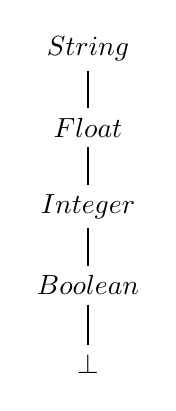
\begin{tikzpicture}

	\node (string)  {$String$};
	\node [below  of=string] (float)  {$Float$};
	\node [below  of=float] (int)  {$Integer$};
	\node [below  of=int] (bool)  {$Boolean$};
	\node [below  of=bool] (bottom)  {$\bot$};
	\draw [thick] (string) -- (float); 
	\draw [thick] (float) -- (int); 
	\draw [thick] (int) -- (bool);
	\draw [thick] (bool) -- (bottom); 
	
	\end{tikzpicture}
\end{center}

In section \ref{concrete} we define $ \mathcal{S} $ to be the set of all possible strings. Here we define the sets $ \mathbb{F}, \mathbb{I}, \mathbb{B} \subseteq \mathcal{S} $ to be the sets of strings that can be interpreted as floating-point numbers, integers and booleans respectively. Then we define a concretization function $ \gamma_{\mathbf{T}}: \mathbf{T} \longrightarrow \mathcal{S} $ for the type lattice as follows: 
\begin{center}
 $ \gamma_{\mathbf{T}}(String) = \mathcal{S} $ \\
 $ \gamma_{\mathbf{T}}(Float) = \mathbb{F} $ \\
  $ \gamma_{\mathbf{T}}(Integer) = \mathbb{I} $ \\
   $ \gamma_{\mathbf{T}}(Boolean) = \mathbb{B} $ \\
    $ \gamma_{\mathbf{T}}(\bot) = \phi $

\end{center}
The operators $ \sqsubseteq_{\mathbf{T}}, \sqcup_{\mathbf{T}}, \sqcap_{\mathbf{T}} $ can be defined using the Hass diagram above. \\

We define arithmetic operations for the type lattice as follows:\\
\hspace*{15mm}$ t_{1} + t_{2}$ = $ \left\{
\begin{array}{ll}
Integer & t_{1} = Boolean \wedge t_{2} = Boolean \\
String & t_{1} = String \wedge t_{2} = String \\
\bot_{\mathbf{T}} & (t_{1} = String \wedge t_{2} \neq String) \vee (t_{1} \neq String \wedge t_{2} = String) \\
t_{1} \sqcup_{\mathbf{T}} t_{2} & otherwise
\end{array} 
\right. $ \\ \\

\hspace*{10mm}$ t_{1} - t_{2}$ = $ \left\{
\begin{array}{ll}
Integer & t_{1} = Boolean \wedge t_{2} = Boolean \\
\bot_{\mathbf{T}} & t_{1} = String \vee  t_{2} = String \\
t_{1} \sqcup_{\mathbf{T}} t_{2} & otherwise
\end{array} 
\right. $ \\ \\

\hspace*{10mm}$ t_{1} \times t_{2}$ = $ \left\{
\begin{array}{ll}
Integer & t_{1} = Boolean \wedge t_{2} = Boolean \\
\bot_{\mathbf{T}} & t_{1} = String \wedge  (t_{2} = String \vee t_{2} = Float) \\
\bot_{\mathbf{T}} & t_{2} = String \wedge  (t_{1} = String \vee t_{1} = Float) \\
t_{1} \sqcup_{\mathbf{T}} t_{2} & otherwise
\end{array} 
\right. $ \\ \\

\hspace*{10mm}$ t_{1} \div t_{2}$ = $ \left\{
\begin{array}{ll}
 \bot_{\mathbf{T}} & t_{1} = Boolean \vee t_{2} = Boolean \\
	Float & otherwise
\end{array} 
\right. $ \\ \\
 
To define the Type Domain, we assume that a static type inference has already been run on the program and that it infers the most generic type for a variable in all execution paths of the program. Our Type Domain aims to track more fine-grained information about the types of variables. We assume that the function $ \mathtt{type}(v) $ returns the type of a variable according to the type inference. Then we proceed to define the Type Domain as follows: 

\begin{center}
	$ \mathrm{TYP} \equiv \mathcal{V} \longrightarrow \mathbf{T}$
\end{center} 
\begin{itemize}
	\item An element $ t \in \mathrm{TYP} = \lbrace v \rightarrow typ\ \vert\ v \in \mathcal{V} \wedge typ \in \mathbf{T}  \rbrace $. An element of this domain maps a variable to an element of the type lattice. 
	\item A concretization function $ \gamma_{\mathbf{TYP}} $:
	\begin{itemize} 
		\item We first define a function $ \gamma_{c}: (\mathcal{V} \rightarrow \wp(\mathcal{S})) \longrightarrow \wp(\mathcal{V} \rightarrow \mathcal{S}) $, which transforms a mapping from variable to multiple string values to multiple mappings from a variable to a string value. 
		\item We define an intermediate concretization function $ \gamma'_{\mathbf{TYP}}: \mathrm{TYP} \longrightarrow (\mathcal{V} \rightarrow \wp(\mathcal{S})) $ as follows: $ \gamma'_{\mathrm{TYP}}(f) = \lambda_{x}\cdot \gamma_{\mathbf{T}}(f(x)) $. 
		\item Finally, the concretization function of the Type Domain $ \gamma_{\mathrm{TYP}}: \mathrm{TYP} \longrightarrow \wp(\mathcal{V} \rightarrow \mathcal{S}) $ as the chaining of the two previous functions: $ \gamma_{c} \circ \gamma'_{\mathrm{TYP}}$. It maps every variable to the possible values it can take according to its type. 
	\end{itemize}
\item A partial order $ \sqsubseteq_{\mathrm{TYP}} $: $ t_{1} \sqsubseteq_{\mathrm{TYP}} t_{2} \Longleftrightarrow \forall_{v \in \mathcal{V}} (t_{1}(v) \sqsubseteq_{\mathbf{T}} t_{2}(v))$. For an element of the domain to be smaller than the other, it has to the case that it maps every variable involved in the program to a smaller lattice element than it is mapped in the other element. 
\item A minimum element $ \bot_{\mathrm{TYP}} = \lambda_{x} \cdot \bot_{\mathbf{T}}$. It simply maps every variable to the least element of the type lattice. This represents a type error state. 
\item A maximum element $ \top_{\mathrm{TYP}} = \lambda_{x} \cdot \mathtt{type}(x) $. Since the type inference calculates the most generic type a variable can take, the maximum element of this domain maps every variable to the type computed for it by the type inference. If a variable has a type Float in the type inference, then this it the most generic it can have in all paths of the program and therefore we do not assign it to String but to Float. 
\item A join operator $ \sqcup_{\mathrm{TYP}} $: $ t_{1} \sqcup_{\mathrm{TYP}} t_{2} = \lambda_{x}\cdot t_{1}(x) \sqcup_{\mathbf{T}} t_{2}(x) $. If variable is mapped to two different types in two different paths, then, when these paths are joined, we map the variable to the more \textit{generic} type. That is, the type that is higher in the type lattice Hass diagram. 

\item A meet operator $ \sqcap_{\mathrm{TYP}} $: $ t_{1} \sqcap_{\mathrm{TYP}} t_{2} = \lambda_{x}\cdot t_{1}(x) \sqcap_{\mathbf{T}} t_{2}(x) $.
\item A backward assignment operator $ \llbracket X:=aexpr \rrbracket(t) = \mathrm{SUBS}_{\mathrm{TYP}}(t, X, aexpr)$ which is described in Algorithm \ref{subsT}. The substitution algorithm evaluates $ aexpr $ and all its sub-expressions and then refines the state $ t $ using this evaluation and the type of $ X $. 
\item A filter operator $ \llbracket cond \rrbracket(t) = t $. It does not affect the state.
\item A widening operator $ \nabla_{\mathrm{TYP}} \equiv \sqcup_{\mathrm{TYP}} $. 

We note that since the Type Domain is a non-relational domain, a replacement operator $ \mathcal{R}_{\mathrm{TYP}} $ and a unification operator $ \mathcal{U}_{\mathrm{TYP}} $ return the state unchanged. 

\end{itemize}

	
	\begin{algorithm}[H]
		\caption{Substitution algorithm for Type Domain} \label{subsT}
		\begin{algorithmic}
			\Function{$ \mathrm{SUBS}_{\mathrm{TYP}} $} {$t,\  x,\ aexpr $}
			
			\State $ value \gets t(x) $
			\State $ t(x) \gets \mathtt{type}(x) $
			\State $ eval \gets empty\ map $
			\State $ eval \gets \mathrm{EVAL}_{\mathrm{TYP}}(aexpr, eval) $
			\State $ \mathrm{REFINE}_{\mathrm{TYP}}(aexpr, eval, eval[x] \sqcap_{\mathbf{T}} value, t) $
			\State \Return $ t $
			\EndFunction
		\end{algorithmic}
	\end{algorithm}


\begin{algorithm}[H]
	\caption{Expression evaluation for Type Domain} \label{evalT}
	\begin{algorithmic}
		\Function{$ \mathrm{EVAL}_{\mathrm{TYP}} $} {$ expr, eval $}
		
		\If {$expr$ is a literal}
		\State $ eval[expr] \gets $ type of literal
		\State \Return $ eval $
		\EndIf
		
		\If {$ expr \in \mathcal{V}$}
		\State $ eval[expr] \gets \mathtt{type}(v)$
		\State \Return $ eval $
		\EndIf
		
		\If {$ expr = expr1 \diamond expr2\ \textbf{where}\ \diamond \in \lbrace +, -, \times, \div \rbrace $}
		\State $ eval[expr] \gets \mathrm{EVAL}_{\mathrm{TYP}}(expr1) \diamond \mathrm{EVAL}_{\mathrm{TYP}}(expr2)$
		\State \Return $ eval $
		\EndIf
		
		\EndFunction
	\end{algorithmic}
\end{algorithm}

\begin{algorithm}[H]
	\caption{Expression refinement for Type Domain} \label{refineT}
	\begin{algorithmic}
		\Function{$ \mathrm{REFINE}_{\mathrm{TYP}} $} {$ expr, eval, value, t$}
		
		\If {$ expr $ is a literal}
		\State \Return t
		\EndIf
		
		\If {$ expr \in \mathcal{V}$}
		\State $ t(x) \gets eval[expr] \sqcap_{\mathbf{T}} value$
		\State \Return $ t $
		\EndIf
		
		\If {$ expr = expr1 \diamond expr2\ \textbf{where}\ \diamond \in \lbrace +, -, \times, \div \rbrace $}
		\State $ value \gets eval[expr] \sqcap_{\mathbf{T}} value  $
		\State $ refine1 \gets \mathrm{REFINE}_{\mathrm{TYP}}(expr1, eval, value, t) $
		\State $ refine2 \gets \mathrm{REFINE}_{\mathrm{TYP}}(expr2, eval, value, refine1) $
		\State \Return $ refine2 $
		\EndIf
		
		\EndFunction
	\end{algorithmic}
\end{algorithm}

\subsection{The Octagon Domain} \label{octagon}

The Octagon Domain was introduced by Antoine Min\'{e} in \cite{octagon} as a numerical relational domain that can keep track of relations the form $ \pm X \pm Y \geq c $ where $ X $ and $ Y $ are program variables. We use the Octagon Domain in our analysis in order to keep track of relations between variables such as $ sequence\_length \leq max\_length $ in Listing 2.1. 

As explained in section \ref{sub-domains}, in order for an existing domain to work with our analysis framework, it needs to define a \textit{replacement} operator that, whenever an input is read, introduces a new variable to denote this input and the constraints and relations associated with it before it is stored in the stack. In the same section, we also explain the need to define a unification operator to address the problem of inconsistent environments arising from introducing new variables into our analysis. 

 \begin{lstlisting} [language=Python, caption= Example of Unification] 
x: int = input()
if x > 10:
	y: int = int(input())
	if y + x <= 10:
		raise ValueError
else:
	z: float = float(input())
	if z + x <= 20:
		raise ValueError
\end{lstlisting}

We define a replacement operator $ \mathcal{R}_{O}(o, v, l_{i}) $ for the Octagon Domain, where $ o $ is an octagon, $ v $ is the variable that is being read as input and $ l_{i} $ is the program point at which the input is being read. The operator works by first adding the variable $ l_{i} $ to the octagon. This variable has no constraints associated with it at first. Then, assuming the Octagons Domain defines a backward assignment operator, we perform the substitution $ \llbracket v := l_{i} \rrbracket_{O} $. Thus, $ v $ is replaced by $ l_{i} $ in all the constraints of the octagon and $ v $ becomes top. 


We define the unification operator $ \mathcal{U}_{O}(o_{1}, o_{2}) $ where both $ o_{1} $ and $ o_{2} $ are octagons. The operator is applied before every join, meet or widening operation in the analysis. We assume every element of the Octagon Domain keeps a list of its variables in the order in which they were added during the analysis. For every variable $ l_{i} $ in $ o_{1} $ and $ l_{j} $ in $ o_{2} $, that have the same order in the respective variable lists, if $ j < i $, we replace $ l_{i} $ with $ l_{j} $ in $ o_{1} $. That is, when we have two variables that represent inputs read in the same order in two different paths in the analysis, we replace the variable that represents a later program point, with a variable that represents an earlier program point. After this step, if there are variables in $ o_{2} $ which are not in $ o_{1} $, they are added to $ o_{1} $. Note that in this case the operator is asymmetric and needs to be called twice, $ \mathcal{U}_{O}(o_{1}, o_{2}) $ and $ \mathcal{U}_{O}(o_{2}, o_{1}) $, before every join, meet and widening. 


To illustrate the replacement and unification operators we introduce Listing 2.2. In the then-branch of the if-statement, we read a variable $ y $ and assert the condition $ y + x > 10 $. In the else-branch, we read a variable $ z $ and enforce the condition $ z + x > 20 $. If we trace a backward analysis on this program and employing the $ \mathcal{R}_{O} $ we defined earlier in this section, then in the then-branch, we get $\mathcal{R}_{O}(\lbrace y + x > 10\rbrace, y, l_{3}) = \lbrace l3 + x > 10 \rbrace$ and similarly in the else-branch we get the relation $ \lbrace l_{7} + x > 20 \rbrace$. A join needs to be performed on these two elements at the head of the if-statement. Since our analysis treats $ l_{3} $ and $ l_{7} $ as different variables, without the unification operator, the join will yield top. 

 As mentioned earlier, our analysis does not care about the specific variables representing input values, but rather about the order in which they occur in the list of input values which the program reads in their respective paths. In this example, we only care that after reading $ x $ we read another variable whose summation to $ x $ had to be greater than 20, otherwise the program will crash. Therefore, for the purpose of our analysis, $ l_{3} $  and $ l_{7} $ should be treated as the same variable when joining the two paths at the head of the if-condition since both of them are read second in their respective paths. We call the unification operator once as follows: $ \mathcal{U}_{O}(\lbrace l_{3} + x > 10 \rbrace, \lbrace l_{7} + x > 20 \rbrace) =  \lbrace l_{3} + x > 10 \rbrace$ and then another time switching the operands as follows: $ \mathcal{U}_{O}(\lbrace l_{7} + x > 20 \rbrace, \lbrace l_{3} + x > 10 \rbrace) =  \lbrace l_{3} + x > 20 \rbrace$. Then a join can be performed between $ \lbrace l_{3} + x > 10 \rbrace $ and $ \lbrace l_{3} + x > 20 \rbrace $ which will give us $ l_{3} + x > 20 $. 

\subsection{The Character Inclusion Domain} \label{character}
The Character Inclusion Domain, as defined in \cite{character}, is an abstract domain that maps a string into two sets: a set of characters that are certainly included in the string and another set of characters that may be included in the string. 
For a finite alphabet $\mathrm{A}$, we define a character inclusion lattice as follows: 
\begin{itemize}
	\item An element $c \in CI = \lbrace(C, M): C, M \in \wp (\mathrm{A}) \land C \subseteq M \rbrace \cup \bot_{CI}$. This can be understood as an abstraction of a string which certainly contains all the characters in $C$ and is only allowed to contain characters in $ M $.
	
	\item A concretization function $\gamma_{CI}$: $\langle CI, \sqsubseteq_{CI}\rangle  \longrightarrow \langle A^{*}, \subseteq\rangle$ such that \\ $ \gamma_{CI}((C, M)) = \lbrace x\ \vert\ x \in A^{*} \wedge \mathtt{char}(x) \supseteq C \wedge \mathtt{char}(x) \subseteq M \rbrace $, where $ \mathtt{char}(x) $ is a function that returns the set of all characters in a string  $ x $.  An element $ (C, M) $ concertizes to the set of all string which contain all the characters in $ C $ and which do not contain any characters outside $ M $. 
	
	\item A partial order: $(C_{1}, M_{1}) \sqsubseteq_{CI} (C_{2}, M_{2}) \iff (C_{1} \supseteq C_{2}, M_{1} \subseteq M_{2})$. This order indicates that the fewer the certainly included characters and the more the maybe included characters, the more strings we represent. For example the element $(\lbrace a \rbrace , \lbrace a,b \rbrace)$ concertizes to $\lbrace a, aa, ab, aaa, aab,... \rbrace$ while the element $(\emptyset, \lbrace a, b \rbrace)$ concertizes to $\lbrace\varepsilon, a, b, aa, ab, bb,...\rbrace$. The restriction of having $a$ in the certainly included set makes the values $\lbrace \varepsilon, b, bb, bbb,...\rbrace $ disappear from the concretization. 
	
	\item A least element $\bot_{CI}$ which represents a failure state. 
	\item A greatest element $\top_{CI} = (\emptyset, A) $ which represents a string that can contain any combination of characters from the alphabet. 
	
	\item A join operator: $(C_{1}, M_{1}) \sqcup_{CI} (C_{2}, M_{2}) = (C_{1} \cap C_{2}, M_{1} \cup M_{2})$. The soundness of this operator can be stated as follows: \\ $ \lbrace x\ \vert\ x \in A^{*} \wedge \mathtt{char}(x) \supseteq C_{1} \wedge \mathtt{char}(x) \subseteq M_{1} \rbrace \cup \lbrace x\ \vert\ x \in A^{*} \wedge \mathtt{char}(x) \supseteq C_{2} \wedge \mathtt{char}(x) \subseteq M_{2} \rbrace \subseteq  \lbrace x\ \vert\ x \in A^{*} \wedge \mathtt{char}(x) \supseteq C_{1}\ \cap\ C_{2}\ \wedge\ \mathtt{char}(x) \subseteq M_{1} \cup M_{2} \rbrace \Longleftrightarrow \gamma_{CI}((C_{1}, M_{1})) \cup \gamma_{CI}((C_{2}, M_{2})) \subseteq \gamma_{CI}((C_{1}, M_{1}) \sqcup_{CI} (C_{2}, M_{2}))$. If we have two elements $ (\lbrace a, b \rbrace, \lbrace a, b, c \rbrace) $ and $ (\lbrace a \rbrace, \lbrace a, b, d \rbrace) $ that we would like to join, then we can only say that the resulting element will \textit{certainly} contain the character $ a $ (the intersection of $ C $ sets), but it \textit{may} contain any of the characters $ a,\ b,\ c\ $ or $ d $ (the union of the two $ M $ sets). 
	
	 
	\item A meet operator: $(C_{1}, M_{1}) \sqcap_{CI} (C_{2}, M_{2}) = (C_{1} \cup C_{2}, M_{1} \cap M_{2}) \cup \bot_{CI}$. The bottom is to account for cases when $C_{1} \cup C_{2} \not\subseteq M_{1} \cap M_{2}$. The soundness of this operator can be stated as follows: \\$ \lbrace x\ \vert\ x \in A^{*} \wedge \mathtt{char}(x) \supseteq C_{1} \wedge \mathtt{char}(x) \subseteq M_{1} \rbrace \cap \lbrace x\ \vert\ x \in A^{*} \wedge \mathtt{char}(x) \supseteq C_{2} \wedge \mathtt{char}(x) \subseteq M_{2} \rbrace \subseteq  \lbrace x\ \vert\ x \in A^{*} \wedge \mathtt{char}(x) \supseteq C_{1} \cup C_{2} \wedge \mathtt{char}(x) \subseteq M_{1} \cap M_{2} \rbrace \Longleftrightarrow \gamma_{CI}((C_{1}, M_{1})) \cap \gamma_{CI}((C_{2}, M_{2})) \subseteq \gamma_{CI}((C_{1}, M_{1}) \sqcap_{CI} (C_{2}, M_{2}))$. The meet works in the opposite way to the join. If we have two elements $ (\lbrace a, b \rbrace, \lbrace a, b, c \rbrace) $ and $ (\lbrace a \rbrace, \lbrace a, b, d \rbrace) $ which we would like to meet, we can say that the resulting element will \textit{certainly} contain both $ a $ and $ b $ (the union of the two $ C $ sets) and that it \textit{may} contain only $ a $ and $ b $ (the intersection of the two $ M $ set) as well.  
 	
	\item A concatenation operator: $ ((C_{1}, M_{1}) +_{CI} (C_{2}, M_{2})) = ((C_{1} \cup M_{1}),(C_{2} \cup M_{2}))$. When concatenating two string, the resulting string will \textit{certainly} that characters that are certainly included in both strings and \textit{may} contain the characters that may be included in both strings as well. 
	\item A widening operator $\nabla_{CI} \equiv \sqcup_{CI}.$ The widening operator is the same as the join. 
	
\end{itemize}

	Then we define the Character Inclusion Domain as a mapping from variables to elements of the character inclusion lattice as follows: 
\begin{center}
	$ \mathrm{CHAR} \equiv \mathcal{V} \longrightarrow CI $
\end{center} 
\begin{itemize}
	\item An element $ c \in CHAR = \lbrace v \longrightarrow ci\ \vert\  v \in \mathcal{V} \wedge ci \in CI \rbrace $. Every element in the Character Inclusion Domain maps a variable to an element in the character inclusion lattice. 
	\item A concretization function $ \gamma_{\mathrm{CHAR}} $: 
		\begin{itemize} 
		\item We first define a function $ \gamma_{c}: (\mathcal{V} \rightarrow \wp(\mathcal{S})) \longrightarrow \wp(\mathcal{V} \rightarrow \mathcal{S}) $, which transforms a mapping from variable to multiple string values to multiple mappings from a variable to a string value. 
		\item We define an intermediate concretization function $ \gamma'_{\mathrm{CHAR}}: \mathrm{CHAR} \longrightarrow (\mathcal{V} \rightarrow \wp(\mathcal{S})) $ as follows: $ \gamma'_{\mathrm{CHAR}}(f) = \lambda_{x}\cdot \gamma_{CI}(f(x)) $. 
		\item Finally, we define the concretization function of the Character Inclusion Domain $ \gamma_{\mathrm{CHAR}}: \mathrm{CHAR} \longrightarrow \wp(\mathcal{V} \rightarrow \mathcal{S}) $ as the chaining of the two previous functions: $ \gamma_{c} \circ \gamma'_{\mathrm{CHAR}}$. 
	\end{itemize}

	\item A partial order $ \sqsubseteq_{\mathrm{CHAR}} $: $ c_{1} \sqsubseteq_{\mathrm{CHAR}} c_{2} \Longleftrightarrow \forall_{v \in \mathcal{V}} (c_{1}(v) \sqsubseteq_{CI} c_{2}(v))$.
	\item A minimum element $ \bot_{\mathrm{CHAR}} = \lambda_{x} \cdot \bot_{CI}$. Every variable is mapped to the smallest element in the character inclusion lattice.  
	\item A maximum element $ \top_{\mathrm{CHAR}} = \lambda_{x} \cdot \top_{CI} $. Every variable is mapped to the biggest element of the character inclusion lattice. 
	\item A join operator $ \sqcup_{\mathrm{CHAR}} $: $ c_{1} \sqcup_{\mathrm{CHAR}} c_{2} = \lambda_{x}\cdot c_{1}(x) \sqcup_{CI} c_{2}(x) $ which maps a variable to the joining of the two lattice elements to which it was mapped in $ c_{1} $ and $ c_{2} $.
	 
	\item A meet operator $ \sqcap_{\mathrm{TYP}} $: $ c_{1} \sqcap_{\mathrm{CHAR}} c_{2} = \lambda_{x}\cdot c_{1}(x) \sqcap_{CI} c_{2}(x) $ which maps a variable to the meet of the two lattice elements to which it was mapped in $ c_{1} $ and $ c_{2} $. 
	\item A backward assignment operator $ \llbracket X:=aexpr \rrbracket(c) = \mathrm{SUBS}_{\mathrm{CHAR}}(c, X, aexpr)$ which is described in Algorithm \ref{subsC}. It evaluates $ aexpr $ and all its sub-expressions and refine the state $ c $ with the values computed in this evaluation and the value to which $ X $ was mapped before the assignment is invoked. Meanwhile, $ X $ becomes top.
	
	\item A filter operator $ \llbracket cond \rrbracket(c) =  \mathrm{FILTER}_{\mathrm{CHAR}}(cond, c)$ which is described in Algorithm \ref{filterC}.
	\item A widening operator $ \nabla_{\mathrm{CHAR}} \equiv \sqcup_{\mathrm{CHAR}} $ which is equivalent to the join. 

\end{itemize}
 
As is the case for the Type Domain, the replacement operator $ \mathcal{R}_{\mathrm{CHAR}} $ and a unification operator $ \mathcal{U}_{\mathrm{CHAR}} $ do not produce any changes on the state since this domain is non-relational. 

\begin{algorithm}[H]
	\caption{Substitution algorithm for Character Inclusion Domain} \label{subsC}
	\begin{algorithmic}
		\Function{$ \mathrm{SUBS}_{\mathrm{CHAR}} $} {$c,\  x,\ aexpr $}
		
		\State $ value \gets c(x) $
		\State $ c(x) \gets \top_{CI} $
		\State $ eval \gets emtpy\ map$
		\State $ eval \gets \mathrm{EVAL}_{\mathrm{CHAR}}(aexpr, eval, c) $
		\State $ \mathrm{REFINE}_{\mathrm{CHAR}}(aexpr, eval, eval[x] \sqcap_{CI} value, c) $
		\State \Return $ c $
		\EndFunction
	\end{algorithmic}
\end{algorithm}

\begin{algorithm}[H]
	\caption{Filter algorithm for Character Inclusion Domain} \label{filterC}
	\begin{algorithmic}
		\Function{$ \mathrm{FILTER}_{\mathrm{CHAR}} $} {$cond,\ c$}
		\If {$ cond = (cond1 \wedge cond2) $}
		\State $ c1 \gets \mathrm{FILTER}_{\mathrm{CHAR}}(cond1, c)$
		\State $ c2 \gets \mathrm{FILTER}_{\mathrm{CHAR}}(cond2, c)$
		\State \Return $ c1 \sqcap_{\mathrm{CHAR}} c2$
		\ElsIf {$ cond = (cond1 \vee cond2) $}
		\State $ c1 \gets \mathrm{FILTER}_{\mathrm{CHAR}}(cond1, c)$
		\State $ c2 \gets \mathrm{FILTER}_{\mathrm{CHAR}}(cond2, c)$
		\State \Return $ c1 \sqcup_{\mathrm{CHAR}} c2$
		\ElsIf {$ cond = (expr1 == expr2) $}
		\State $ eval1 \gets empty\ map $
		\State $ eval1 \gets \mathrm{EVAL}_{\mathrm{CHAR}}(expr1, eval1, c) $
		\State $ eval2 \gets empty\ map $
		\State $ eval2 \gets \mathrm{EVAL}_{\mathrm{CHAR}}(expr2, eval2, c) $
		\State $ \mathrm{REFINE}_{\mathrm{CHAR}}(expr1, eval1, eval1[expr1], c)$
		\State $ \mathrm{REFINE}_{\mathrm{CHAR}}(expr2, eval2, eval2[expr2], c)$
				
		\EndIf
		\State \Return $ c $
		\EndFunction
	\end{algorithmic}
\end{algorithm}

\begin{algorithm}[H]
	\caption{Expression evaluation for Character Inclusion Domain} \label{evalC}
	\begin{algorithmic}
		\Function{$ \mathrm{EVAL}_{\mathrm{CHAR}} $} {$ expr, eval, c $}
		
		\If {$expr$ is a literal}
		\State $ eval[expr] \gets (\mathtt{char}(x), \mathtt{char}(x) )$ 
		\State \Return $ eval $
		\EndIf
		
		\If {$ expr \in \mathcal{V}$}
		\State $ eval[expr] \gets c(expr)$
		\State \Return $ eval $
		\EndIf
		
		\If {$ expr = expr1 + expr2$}
		\State $ eval[expr] \gets \mathrm{EVAL}_{\mathrm{CHAR}}(expr1) +_{CI} \mathrm{EVAL}_{\mathrm{CHAR}}(expr2)$
		\State \Return $ eval $
		\EndIf
		
		\EndFunction
	\end{algorithmic}
\end{algorithm}

\begin{algorithm}[H]
	\caption{Expression refinement for Character Inclusion Domain} \label{refineC}
	\begin{algorithmic}
		\Function{$ \mathrm{REFINE}_{\mathrm{CHAR}} $} {$ expr, eval, (C, M), c$}
		
		\If {$ expr $ is a literal}
		\State \Return c
		\EndIf
		
		\If {$ expr \in \mathcal{V}$}
		\State $ c(x) \gets eval[expr] \sqcap_{CI} (C, M)$
		\State \Return $ c $
		\EndIf
		
		\If {$ expr = expr1 + expr2 $}
		\State $ (C, M) \gets eval[expr] \sqcap_{CI} (C, M)  $
		\State $ refine1 \gets \mathrm{REFINE}_{\mathrm{TYP}}(expr1, eval, (\emptyset, M), c) $
		\State $ refine2 \gets \mathrm{REFINE}_{\mathrm{TYPE}}(expr2, eval, (\emptyset, M), refine1) $
		\State \Return $ refine2 $
		\EndIf
		
		\EndFunction
	\end{algorithmic}
\end{algorithm}


\chapter{Implementation} \label{implementation}

We implemented our static analysis and input checker in Python as an extension to the Lyra project \cite{lyra}. We then implemented a plug-in for IntelliJ IDEA that enables the user to use the analysis and checker as a tool. The plug-in implementation is in Java. 



We implement the Assumption Domain described in section \ref{assumption-domain} in a class we call $ AssumptionState $.  The $ AssumptionState $ class has a list of sub-states which represents the sub-domains in the Assumption Domain. The Type Domain already exists as part of Lyra. We implemented separate classes for the Octagon and Character Inclusion domains. For the Octagon domain, we used the Python interface of the ETH Library for Numerical Analysis (ELINA) \cite{singh}. We added extra logic in order to translate the Lyra representation of expressions and conditions into a representation that is compatible with ELINA and also to implement the replacement and unification operators mentioned in section \ref{octagon}. The Character Inclusion domain is implemented as described in section \ref{character} with the addition of support for built-in python functions that perform checks on the characters included in a string such as \verb|isalpha()|, \verb|isalnum()|, \verb|isdecimal()|, \verb|isdigit()|, \verb|islower()| and \verb|isupper()|. We also added the Sign Domain, which had already exited as a part of Lyra, to our implementation in order to keep track of constraints such as $ x \neq 0 $ which is impossible to track with Octagons. 

Every one of the sub-states keeps track of all program variables. If a variable belongs to a type that the domain cannot handle, then its value will always be top in this domain. Therefore, an integer variable will always be mapped to top in the Character Inclusion Domain and a string variable will never have any constraints on it in the Octagon Domain. We require all sub-states to define functions that convert their constraints into JSON object and parse them back from JSON object. We also require every sub-state to implement an input-checking function that, given a input value read from a file, is able to tell whether this value satisfies the constraints that the sub-state represents or not. 

The class $ InputStack $ also has the stack described in section \ref{stack} which implemented as an extension to the already existing $ Stack $ interface in Lyra. We define the pop and push operators for it as well as the structure of individual stack layers. The stack layer is implemented in the class $ InputLattice $ which represents a list of possibly repeated constraints on the input data (see the set $ I $ in section \ref{stack}) and defines a mechanism for recording assumptions on the top layer as well as for joining lists of assumptions from different paths of the analysis. 

Our implementation follows a hierarchy similar to that used in \cite{madelin}. We implement an $ AssumptionController $ class which acts as the entry point for our tool and takes as input the path to a Python code file and an input data file. This class controls three other classes that are in the layer right below it in the hierarchy: $ AssumptionAnalysis $ which extends the Lyra $ Runner  $ class, $ JSONHandler $ and $ InputChecker $. The $ AnalysisAnalysis $ class is responsible for running a backward static analysis on a given Python program. The $ JSONHandler $ class is responsible for writing the assumptions resulting from the analysis into a JSON file and later reading them back from the JSON file. The $ InputChecker $ runs a checking algorithm an a given input file and produces a list of errors present in the file. 


The analysis starts with an instance of the $ AssumptionState $ class set to top and traverses the program paths backward calling the appropriate functions from the class at every step. The final result of the analysis is stored in the stack of the final state and it is of type $ InputLattice $. When the analysis terminates, the controller retrieves the result and passes it to the $ JSONHandler $ class which writes the assumptions into JSON file by calling the functions defined in every sub-state. For subsequent runs of the controller, it checks if the code of the program has been modified and if it has not been modified, it does not run the analysis again but calls the $ JSONHandler $ to read the assumptions for that program from the existing JSON file and convert them back into an $ InputLattice $ object. The assumptions are then passed to the $ InputChecker $ class along with the input file which is required to be checked for errors. The $ InputChecker $ traverses the input file line by line and checks the value in every line against the corresponding assumption by calling the input-checking functions defined in every sub-state. It produces a dictionary which maps a line number in the input file to a $ CheckerError $ object which contains an appropriate error message describing how the value on this line violates an assumption. 

\begin{figure}[H]
	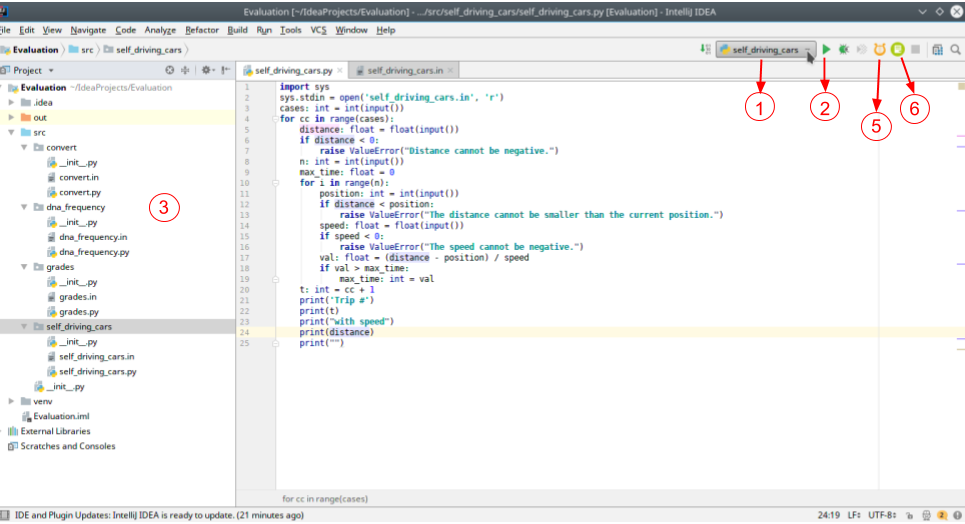
\includegraphics[width=\linewidth]{tool-labeled.png}
	\caption{Screenshot of the IntelliJ IDEA Interface with the Plug-in}
	\label{tool}
\end{figure}

We implement a plug-in for IntelliJ IDEA that allows a user to run our analysis and input checker. The decision to implement such a plug-in was based on feedback received from participants in the user study conducted in \cite{madelin}. The interface which is presented to the user is shown in Figure \ref{tool}. To run the tool on a specific Python program, we must create a run configuration for it and select it from the drop-down menu labeled 1 in the figure. Using the green button labeled 6 we can choose which input data file to check. Then we can run the tool via the button labeled 5 in the figure. The lines which contain errors in the input file will be underlined in red and when the user hovers them with the mouse, an error message will appear. In addition to that, a pop-up message will always appear at the bottom of the screen indicating the location and error message of the first error value in the file. This functionality was added to guide the user step by step in fixing the errors in the file from top to bottom. If the tool cannot detect any more errors in the file, a green pop-up appears at the bottom of the screen indicating so. 
  

\chapter{Evaluation} \label{evaluation}

In this section we present the evaluation of the work done in this thesis. In section \ref{user-study}, we present methodology and result of a user study we conducted in order to evaluate the usability of our tool. In section \ref{analysis-evaluation}, we present an evaluation of the static analysis we defined in section \ref{analysis}. 

\section{User Study} \label{user-study}
We conducted a user study to evaluate the usability of the tool we developed. We asked ten users, five who have a background in computer science and five who study or work in other fields, to use our tool and give us feedback on how helpful they find it. The methodology of the user study is presented in the next section and the results are presented in section \ref{results}. 

\subsection{Methodology} \label{methodology}

In our user study, we asked our users to do two experiments. For every experiment we presented the user with a programs, accompanied by an input data file which contains some errors that will cause the program to crash, and asked them to try to fix the errors in the data file so that the program runs without crashing. For one experiment they were asked to do this without any help and for the other they were asked to do this with the help of our tool. In the sections below we describe the programs and the input data we use and the procedure of the two experiments.

\subsubsection{Programs and Input Data}

We used four programs in our user study. The programs `Grades' (Listing \ref{grades}) and `Self-Driving Cars' (Listing \ref{cars}) are taken from the user study conducted in \cite{madelin}. The programs `Convert' (Listing) and `DNA Frequency' we obtained from the online sources [cite] and [cite] respectively. The code of the programs so that it can be handled by our analysis. For example, we removed statements that contain lists and function call. We also added new statement which provide more interesting assumptions on these input data. We constructed the input datasets to contain an average of eight errors per file. The errors we added can be classified into two main types: errors which appear as a result of typing mistakes, such as the number \textbf{6.5}, which represents a grade, being typed as \textbf{6..5} on line 32 in Listing \ref{grades-data}, and errors which result from some garbage values being printed in the data file due to, for example, the conversion of data from one format to another such as the value \textbf{G}, which represents a DNA base, being printed as \textbf{..G} on line 6 in Listing \ref{dna-data}.   \\ 

\subsubsection{Experiments}
As mentioned earlier, we asked every participant in our user study to do two experiments, one after the other. In both experiments the user was presented with a Python program and a text file containing some input data which has errors that will cause the program to crash. They were asked to not change the code of the program but to change the input data, only adding or modifying lines without deleting them, such that the program runs without crashing. The users were presented with an online form that walked them through the experiments step by step. Before starting the experiments, the users were asked to answer some general questions in the form indicating their age, field of study, current occupation and their level of familiarity with programming on five-point Likert scale ranging from 1 to 5. 

In both experiments, the form explained to them the task that they are required to perform and then asked them to choose one of the four programs based on their month of birth to ensure some randomness in the experiment. They were handed a sheet of paper containing a brief description of the task the program tries to achieve. In the experiment without the tool, they were given instructions on how to run a Python program in IntelliJ IDEA, while in the experiments with the tool, they were given instructions on how to run the tool and what kind of error messages they should expect to see. Then we allowed the user to work on the problem for eight minutes each. Both the form and the problem descriptions are shown in the appendix. 

After every task, we asked the users to answer some questions in the form.  For both experiments we asked if they had been able to fix the errors in the input data and how many minutes they spent on this task. For the experiment with the tool, we added a question about whether or not they were able to run the program without raising any errors. This is to account for the cases were the user was able to fix all the errors detected by the tool, but the tool failed to flag some erroneous data due to imprecision in the analysis.  

These questions were followed by a group of questions on a five-point Likert scale in which the options were: Strongly Disagree, Disagree, Neutral, Agree, Strongly Agree. In both experiments, we asked how frustrated the users felt trying to solve the problems and how understandable they found the error messages printed by the program in the first experiment and displayed by the tool in the second experiment. We added two more questions in the second experiment asking them to rate how user-friendly they found the tool and whether they would rather fix the errors in a data file with or without the help of the tool. 

At the end of the form there were two open-ended questions that aimed to get feedback from the users in their own words. The first questions asked the users what they liked about the tool and the second questions asked them to suggest improvements that they think should be added to the tool. The form as well as the descriptions of the problems can be found in the appendix. 

\subsection{Results} \label{results}

\subsubsection{General questions}

The ages of the participants ranges from 19 to 31 with an average of 23.4. Five participants have backgrounds in computer science (one user used the term "informatics" in the form), while two participants have backgrounds in physics, two in environmental engineering and one in mathematics. Six of our participants are bachelor's students, two are master's students, one participant is a postdoctoral researcher and one is a teaching assistant. 

\begin{lstlisting} [language=Python, label=grades, caption=Code for Program `Grades']
	subject: str = input()
	homeworks: int = int(input())
	students: int = int(input())
	for i in range(students):
		id: str = input()
		sum: float = 0
		max: float = 0
		for j in range(homeworks):
			grade: float = float(input())
			best: float = float(input())
			if grade < 0 or grade > best:
			raise ValueError
			sum: float = sum + grade
			max: float = max + best
		
		average: float = sum / max * 100.0;
		print("Student ID:")
		print(id)
		print("Average homework grade:")
		print(average)
		grade: float = float(input())
		best: float = float(input())
		if grade < 0 or grade > best:
			raise ValueError
		final_grade: float = grade / best * 100.0
		print("Final test grade:")
		print(final_grade)
\end{lstlisting}

\begin{lstlisting} [label=grades-data, caption=Input Data for `Grades']
	CS 101: Introduction to Computer Science
	3
	4
	34-8342
	9
	10
	12
	12
	11
	10
	45
	50
	34-14002
	6
	10
	13
	12
	-9
	10
	51
	50
	31-1234
	5.5
	10
	9
	12
	10#
	10
	-43
	50
	34-2373
	6..5
	10
	11
	12
	7
	10
	48 
\end{lstlisting}

\begin{lstlisting} [language=Python, label=cars, caption=Code for Program `Self-Driving Cars']

cases: int = int(input())
for case in range(cases):
	distance: float = float(input())
	if distance < 0:
		raise ValueError("Distance cannot be negative.")
	n: int = int(input())
	max: float = 0
	for i in range(n):
		position: int = int(input())
		if distance < position:
			raise ValueError("Distance cannot be smaller than the current position.")
		speed: float = float(input())
		if speed < 0:
			raise ValueError("Speed cannot be negative.")
		val: float = (distance - position) / speed
		if val > max:
			max: int = val
	t: int = case + 1
	print("Trip:")
	print(t)
	print("with speed")
	print(distance / max)
	
\end{lstlisting}
\begin{lstlisting} [label=cars-data, caption=Input Data for `Self-Driving Cars]
	4
	10.5
	3
	4
	40
	6
	45.5
	12
	50
	120
	5>>
	25km
	90
	45
	99km/h
	-57
	-123
	76
	130
	1200
	140
	50
	2
	60
	120
	30
	112
	200
	2
	100
	120
	170
\end{lstlisting}

\begin{lstlisting} [language=Python, label=convert, caption= Code Program `Convert'] [H]
items: int = int(input())
if items == 0:
	raise ValueError
for i in range(items):
	name: str = input()
	weight: float = int(input())
	if weight <= 0:
		raise ValueError
	unit: str = input()
	if unit == 'pounds' or unit == 'lb' or unit == 'lbs':
		weight: float = weight * 453.592 * 1e-3
	elif unit == 'ounces' or unit == 'oz' or unit == 'oz.':
		weight: float = weight * 28.35 * 1e-3
	elif unit == 'grams' or unit == 'gms' or unit == 'g':
		weight: float = weight * 1e-3
	elif unit == 'kilograms' or unit == 'kilo' or unit == 'kg':
		pass
	else:
		raise ValueError
	print("Item: " + name)
	print("weight:")
	print(weight)
	print("kg")

	
\end{lstlisting} 

\begin{lstlisting} [label=convert-data, caption=Input Data for `Convert']
	10#
	earphones
	300
	gramx
	stereo set
	0
	kg
	camera tripod
	1@
	qounds
	trolly suitcase
	30
	lbs
	laptop lenovo 5070
	1
	kgs
	laptop lenovo thinkpad
	2>>
	pounds
	12x envelope
	35
	gm.
	bic blue pens 4-piece set
	125
	grams
	travel compass
	50
	grams
	vacuum cleaner
	2#0
	kgs
\end{lstlisting}

\begin{lstlisting}[language=Python, label=dna, caption= Code for Program `DNA Frequency']
	sequences: int = int(input())
	if sequences < 1:
		raise ValueError("Expecting at least one DNA sequence")
	for s in range(sequences):
		length: int = int(input())
		a: int = 0
		c: int = 0
		g: int = 0
		t: int = 0
		for i in range(length):
			base: str = input()
			if base == 'A':
			a: int = a + 1
			elif base == 'C':
			c: int = c + 1
			elif base == 'G':
			g: int = g + 1
			elif base == 'T':
			t: int = t + 1
			else:
			raise ValueError
		separator: str = input()
		if separator == '.' or separator == '#':
			pass
		else:
			raise ValueError
		print("Frequency of A nucleotide:")
		print(a)
		print("Frequency of C nucleotide:")
		print(c)
		print("Frequency of G nucleotide:")
		print(g)
		print("Frequency of T nucleotide:")
		print(t)
		CG_content: float = (c + g) / (a + t + c + g) * 100.0
		print("CG content: ")
		print(CG_content)
		print("%")
\end{lstlisting}

\begin{lstlisting} [label=dna-data, caption=Input Data for `DNA Frequency']
	3..
	10
	A
	O
	C
	..G
	G
	X
	T
	A
	C
	G
	#
	15
	C
	G@
	T
	A
	C
	&C*
	G
	T
	O
	G
	A
	C
	T))
	G
	T
	*
	5
	A
	C
	T
\end{lstlisting}

\section{Evaluation of the Static Analysis} \label{analysis-evaluation}

\chapter{Conclusion and Future Work} \label{conclusion}


\appendix
\chapter{Appendix} 

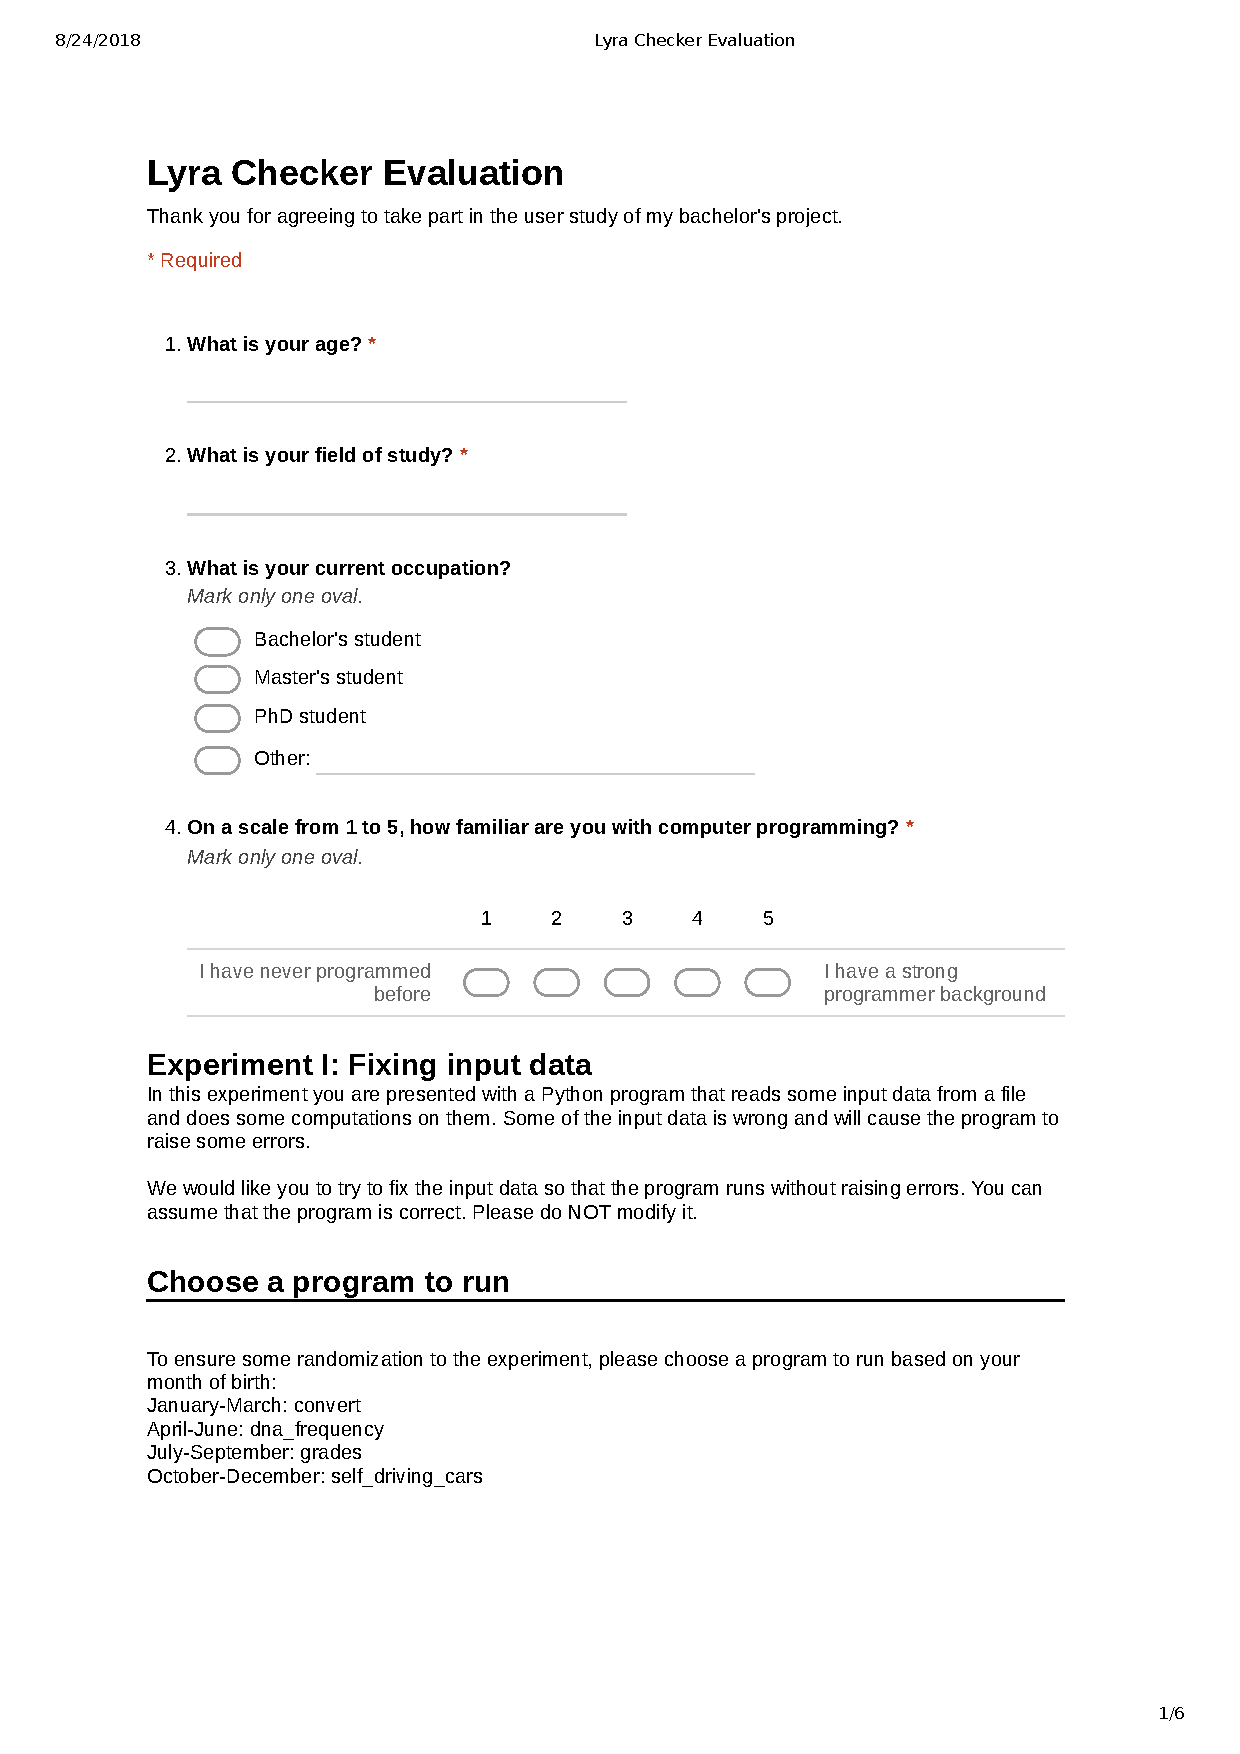
\includepdf[pages={1-6}]{form}

\bibliography{bachelors-thesis}
\bibliographystyle{unsrt}


\end{document}
